% Reproduces plots/mismatch/2_1/hybrid_network_2_1.gml as a TikZ figure.
% Compile with: pdflatex hybrid_network_2_1.tex
\documentclass{article}
\usepackage[margin=1cm]{geometry}
\usepackage{tikz}
\usetikzlibrary{arrows.meta}

% matplotlib tab:blue / tab:orange, matching the gene_color values in the GML
\definecolor{tabblue}{rgb}{0.12156863,0.46666667,0.70588235}
\definecolor{taborange}{rgb}{1.0,0.49803922,0.05490196}

\begin{document}
\thispagestyle{empty}
\begin{center}
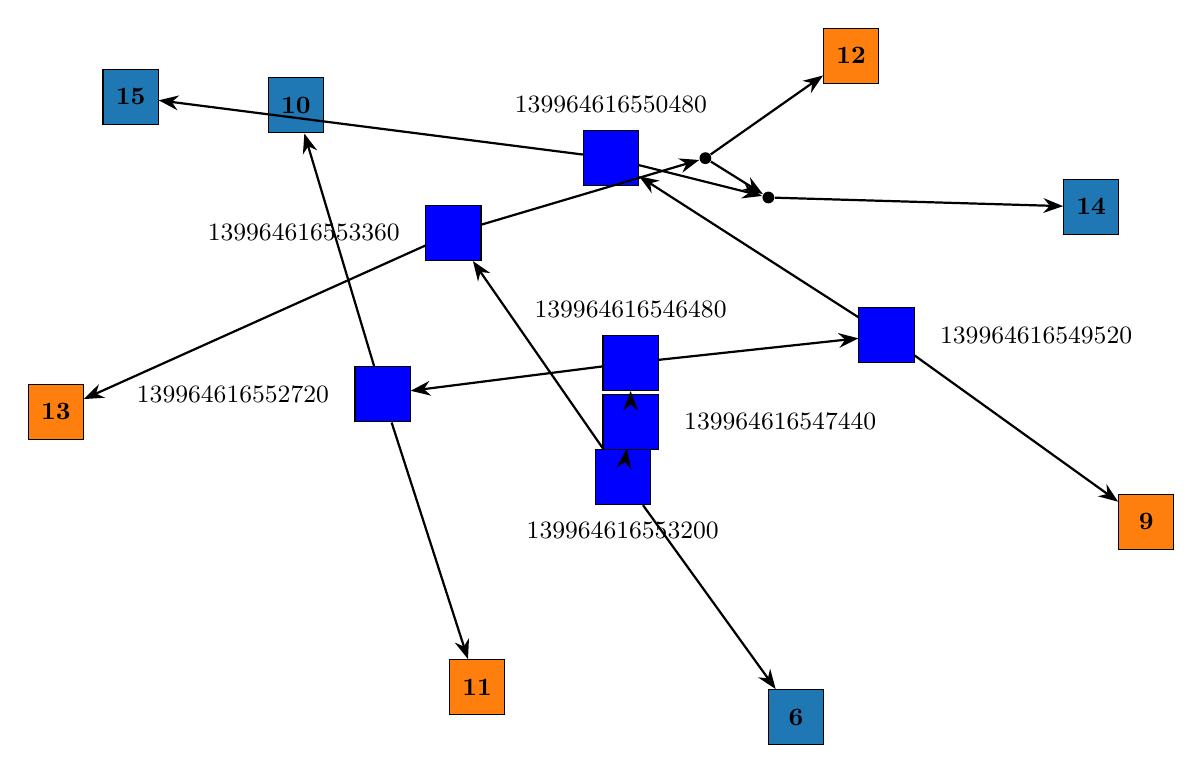
\begin{tikzpicture}[
  >={Stealth[length=2.5mm]},
  every node/.style={font=\small\bfseries},
  internal/.style={rectangle, fill=blue, text=black, minimum size=7mm, draw=black},
  leafblue/.style={rectangle, fill=tabblue, text=black, minimum size=7mm, draw=black},
  leaforange/.style={rectangle, fill=taborange, text=black, minimum size=7mm, draw=black},
  hybrid/.style={circle, fill=black, minimum size=1.5mm, inner sep=0pt},
  edge/.style={->, thick},
]

% ---- internal (blue) nodes: gene-tree/network events ----
\node[internal] (n547440) at (8.05, 4.25) {};
\node[internal] (n546480) at (8.05, 5.00) {};
\node[internal] (n549520) at (11.30, 5.35) {};
\node[internal] (n550480) at (7.80, 7.60) {};
\node[internal] (n552720) at (4.90, 4.60) {};
\node[internal] (n553200) at (7.95, 3.55) {};
\node[internal] (n553360) at (5.80, 6.65) {};

% ---- hybridization / edge-subdivision points (from generateHybridNetwork) ----
\node[hybrid] (hA) at (9.00, 7.60) {};   % h_139964616553360_12_evt0
\node[hybrid] (hB) at (9.80, 7.10) {};   % h_139964616550480_14_evt0

% ---- leaves ----
\node[leafblue]   (l10) at (3.80, 8.27) {10};
\node[leafblue]   (l14) at (13.90, 6.98) {14};
\node[leafblue]   (l15) at (1.70, 8.38) {15};
\node[leafblue]   (l6)  at (10.15, 0.50) {6};
\node[leaforange] (l9)  at (14.60, 2.98) {9};
\node[leaforange] (l11) at (6.10, 0.88) {11};
\node[leaforange] (l12) at (10.85, 8.90) {12};
\node[leaforange] (l13) at (0.75, 4.38) {13};

% ---- labels for internal / hybrid nodes (placed beside the boxes) ----
\node[anchor=west, font=\small]  at ([xshift=2mm]n547440.east)  {139964616547440};
\node[anchor=south, font=\small] at ([yshift=1mm]n546480.north) {139964616546480};
\node[anchor=west, font=\small]  at ([xshift=2mm]n549520.east)  {139964616549520};
\node[anchor=south, font=\small] at ([yshift=1mm]n550480.north) {139964616550480};
\node[anchor=east, font=\small]  at ([xshift=-2mm]n552720.west) {139964616552720};
\node[anchor=north, font=\small] at ([yshift=-1mm]n553200.south) {139964616553200};
\node[anchor=east, font=\small]  at ([xshift=-2mm]n553360.west) {139964616553360};

% ---- edges (exactly as in hybrid_network_2_1.gml) ----
\draw[edge] (n547440) -- (n546480);
\draw[edge] (n547440) -- (n553200);
\draw[edge] (n546480) -- (n549520);
\draw[edge] (n546480) -- (n552720);
\draw[edge] (n549520) -- (n550480);
\draw[edge] (n549520) -- (l9);
\draw[edge] (n550480) -- (l15);
\draw[edge] (n550480) -- (hB);
\draw[edge] (n552720) -- (l10);
\draw[edge] (n552720) -- (l11);
\draw[edge] (n553200) -- (n553360);
\draw[edge] (n553200) -- (l6);
\draw[edge] (n553360) -- (l13);
\draw[edge] (n553360) -- (hA);
\draw[edge] (hA) -- (l12);
\draw[edge] (hA) -- (hB);
\draw[edge] (hB) -- (l14);

\end{tikzpicture}
\end{center}
\end{document}
